
\title{A Primer on the Material Point Method (MPM)}
\author{Rebecca Brannon}
\date{\mydate\today}
\titlepic{\setlength\fboxsep{0pt}\setlength\fboxrule{4pt}
 \fcolorbox{Blue}{Blue}{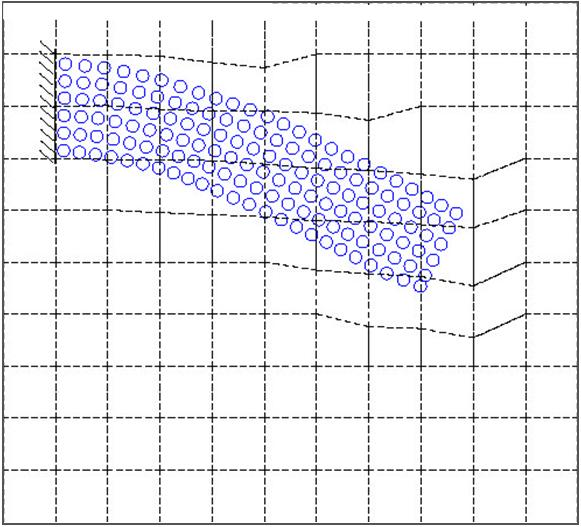
\includegraphics[width=0.3\textwidth]{CoverArtwork}}}
\begin{minipage}[h]{\textwidth}
    \maketitle
\end{minipage}
\vspace{1cm}

\begin{MyAbstract}
\paragraph{ABSTRACT:}
This \manuscript is a beginner's tutorial on the Material Point Method (MPM), which can be viewed as an extension of an updated-Lagrangian finite-element method (FEM) to better accommodate very complicated geometries (like intricate porous micro-structures), as well as extremely large deformations (as seen in penetration) without requiring any remapping or advection schemes for a material model's internal variables. The MPM further provides, at no additional cost, an automatic no-slip/no-stick material contact at locations not known in advance (as in compression of a porous microstructure or sloshing of a fluid).  This primer includes reviews of traditional linear FEM in \oneD, transient nonlinear FEM in \oneD and \twoD.  Following each review of traditional FEM, the revisions in the algorithm required to solve the same problem using MPM are explained.

\end{MyAbstract}






\begin{comment}
\begin{acknowledgements}
The need to write this primer became clear in August 2013, when Steve Schmidt, as student in the Computational Solid Mechanics (CSM) group at the University of Utah asked a well-known MPM researcher, Jim Guilkey, if there were any good books about the MPM.  Jim replied that he was not aware of any good books on this topic. After a pause, he added ``at least there aren't any bad books on MPM either.'' A few minutes later, Steve sent Jim a screenshot of a book advertised by Barnes and Nobel booksellers under the title ``The Material Point Method.''  Within minutes, we realized that the two Russian ``authors'' were known to farm Wikipedia to create ``books'' that they didn't write themselves.  Therefore, thanks go to Barnes and Nobel for their failure to filter out this sort of sleazy publishing, prompting us to try writing an MPM book!
\end{acknowledgements}
\end{comment}


\chapter{A Primer on the Material Point Method (MPM)}
The goal of this tutorial on the Material Point Method (MPM) is to show you how to write your own MPM code, assuming that you already have a finite-element method (FEM) code available to modify (or at least you have sufficient FEM experience to write one as needed). This tutorial does not explain syntax of any particular MPM code, nor does it re-teach the finite-element method. As a tutorial, this \manuscript naturally lacks detailed discourse on the rigorous mathematical foundations of the MPM, but citations are provided pointing to appropriate archival literature \cite{SulskyLoveXXXX}. In a sequence of increasingly complicated example problems, a conventional FEM solution is summarized for each problem, thus forming a starting point from which revisions are then applied to convert an FEM code to an MPM code. Each of these case-study problems finishes with and algorithm and/or pseudo-code for computer implementation, along with at least one verification test problem.